\chapter{Code}
\section{Côté client}
\subsection{Fonctionnement général}
\label{sec:general}
Le client commence sur une ligne noire, qu'il suit jusqu'à un code-barres fait en legos. Il utilise pour cela les deux capteurs infrarouges du dessous avec ce code.
\begin{figure}[H]
  \centering
  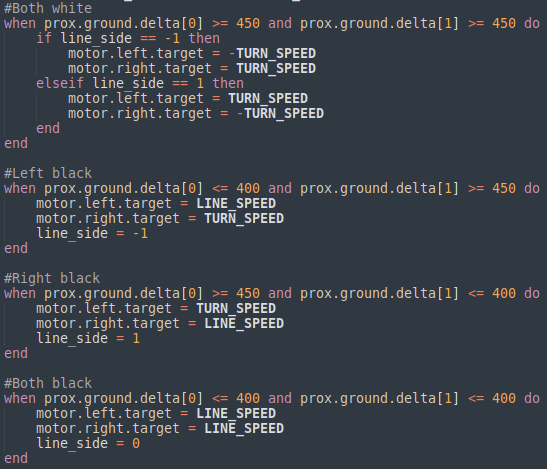
\includegraphics[height=7.1cm]{code/client_line_following}
  \caption{Suivi de la ligne}
  \label{fig:client_line_following}
\end{figure}

Il monte ensuite sur le code-barres et détecte les changements d'angle pour savoir lorsqu'il est de nouveau à plat.

La lecture du code se fait de la manière suivante.
Une première plaque noire permet de définir la longueur d'une barre.
Celle-ci est suivie d'une plaque blanche qui délimite le début du code.
Les barres suivantes représentent la valeur du code en binaire sur 6 bits, où le noir correspond à un 1 et le blanc à un 0.

Le robot calcule les longueurs des différentes zones de couleurs et les divisent par la longueur d'une plaque. (cf. section \ref{sec:barcode})
Afin d'obtenir un résultat optimal, le robot doit préalablement calibrer les capteurs aux couleurs des legos.
Finalement, il convertit la valeur binaire en décimal grâce à la sous-routine suivante.

\begin{figure}[H]
  \centering
  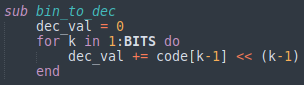
\includegraphics[width=0.8\linewidth]{code/client_bin_to_dec}
  \caption{Binaire -> décimal}
  \label{fig:client_bin_to_dec}
\end{figure}

Une fois le code scanné, le robot redescend puis suit la ligne en direction du serveur.
S'ensuit une discussion par infrarouges entre les deux robots.

Afin qu'ils se comprennent, nous avons dû établir un protocole comme décrit dans l'annexe \ref{app:protocol}.

Tout d'abord, le client émet en continu le message de "handshake". Dès que le serveur le détecte, le processus de communication est entamé (cf. annexe \ref{app:communication}).

Si le serveur est en train de déplacer l'ascenseur, il renvoie la commande "moving", indiquant au client de s'arrêter mais de continuer à émettre le "handshake".

Si après envoi de l'id, le serveur détermine qu'aucune chambre n'est libre, alors il renvoie la commande "goodbye" et le client se met en rouge.

Finalement, si tout se passe correctement, le client s'allume en vert, continue sa route et monte sur la rampe. Il s'arrête un peu après avoir détecté un retour à l'horizontale.

Lorsque l'ascenseur est en mouvement, le client lance un "timeout" qui se réinitialise à chaque fois qu'il détecte un mur passant devant lui. Quand se "timeout" se termine, le client avance pour entrer dans la chambre et s'arrête dès qu'il ne détecte plus de sol.

\subsection{Code-barres}
\label{sec:barcode}

Dans cette section, nous allons détailler la lecture du code-barres. Le schéma suivant explique la procédure de manière graphique:

\begin{figure}[H]
  \centering
  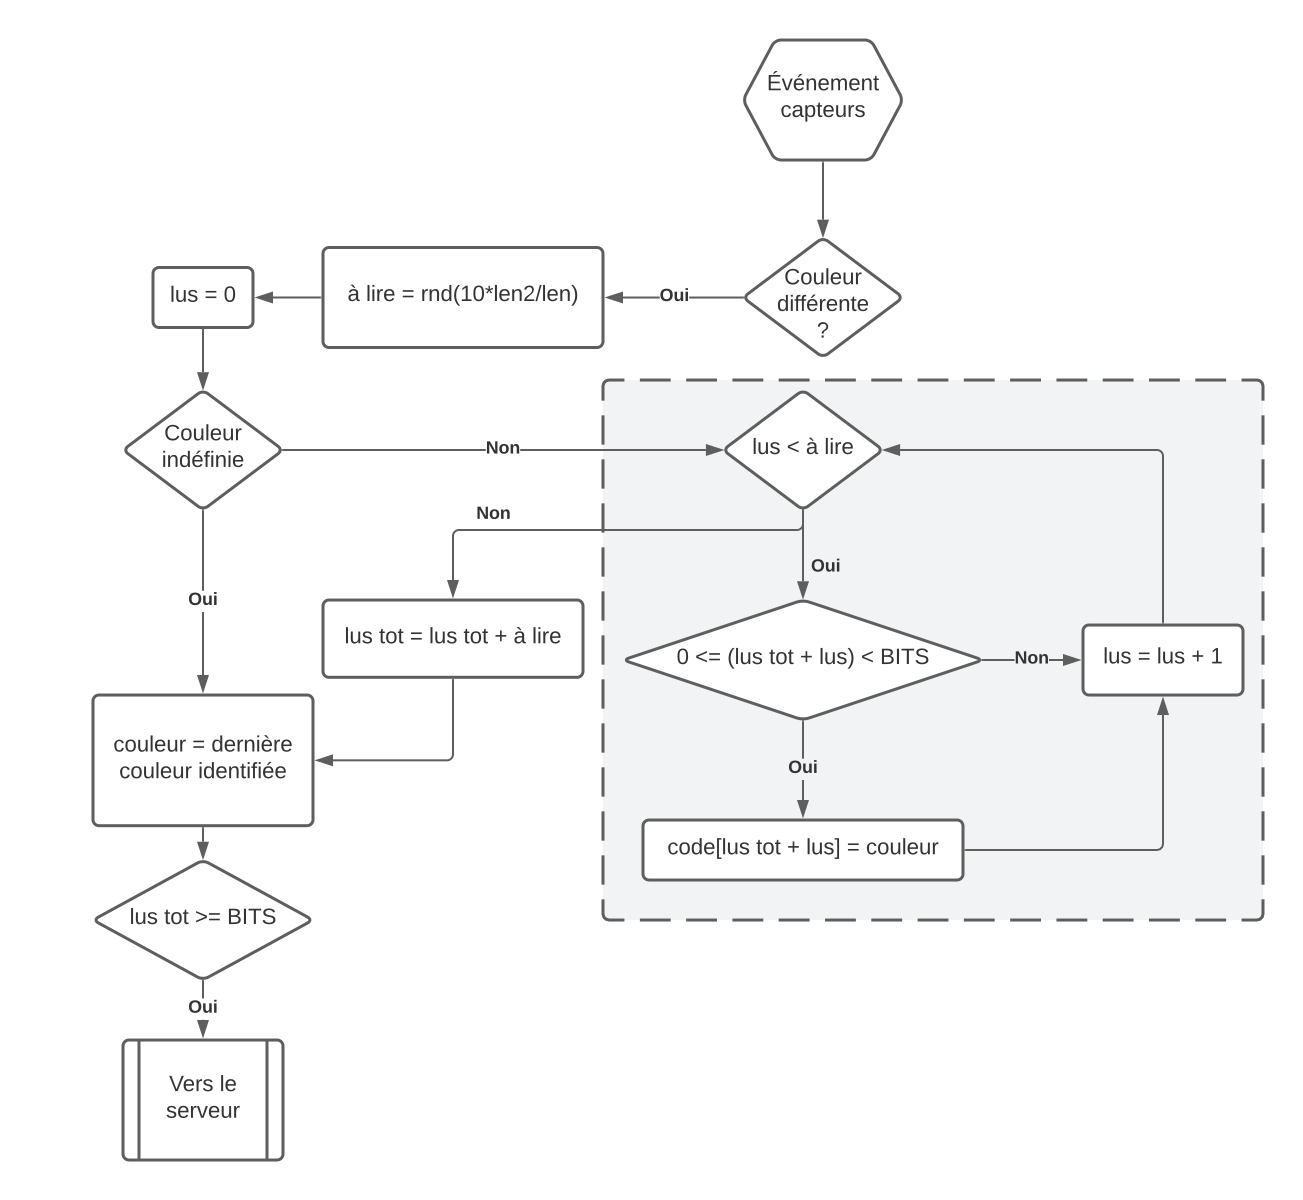
\includegraphics[width=0.9\linewidth]{code/barcode_figure}
  \caption{Lecture du code-barres (schéma)}
  \label{fig:barcode_figure}
\end{figure}

Le point d'entrée est l'événement \texttt{prox} qui est émit en boucle lorsque le robot avance. La couleur sous le robot est identifiée grâce à la sous-routine \texttt{get\_avg} (figure \ref{fig:client_get_avg})

\begin{figure}[H]
  \centering
  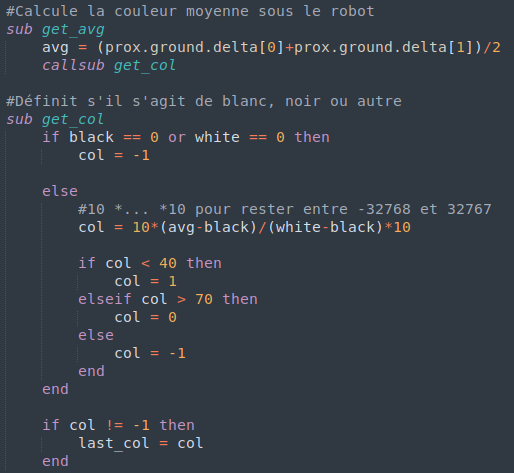
\includegraphics[width=0.7\linewidth]{code/client_get_avg}
  \caption{Calcul de la couleur captée}
  \label{fig:client_get_avg}
\end{figure}

Le robot effectue la lecture à proprement dit à chaque changement de couleur (lorsqu'il passe d'une plaque blanche à une noire et inversément). Sur la figure \ref{fig:barcode_figure}, \texttt{len} est la longueur d'une plaque et \texttt{len2} est la distance parcourue depuis le dernier changement de couleur. Ainsi, \texttt{rnd(len2/len)} est le nombre de plaques constituants cette zone (où \texttt{rnd} est la fonction arrondi).

Si la nouvelle couleur que le robot voit a pu être identifiée, on entre dans la boucle du cadre gris.

Cette boucle rajoute bit à bit la valeur de la couleur dans la liste du résultat, tant que le nombre de plaques lues ne dépasse pas la longueur du code-barres (\texttt{BITS}\footnote{Dans notre cas, \texttt{BITS}=6}). Il s'agit surtout d'une précaution au cas où il ne détecterait pas correctement toutes les plaques lego.

Finalement, le nombre de bits lus jusqu'ici est mis à jour selon le nombre de valeurs ajoutées à cette étape.

Enfin, si le code-barres a été entièrement lu, c'est à dire que le nombre de plaques comptées est supérieur ou égal à la longueur du code, alors le robot passe à l'état \texttt{sTO\_SERVER}.

Ce qui traduit en Aseba donne:
\begin{figure}[H]
  \centering
  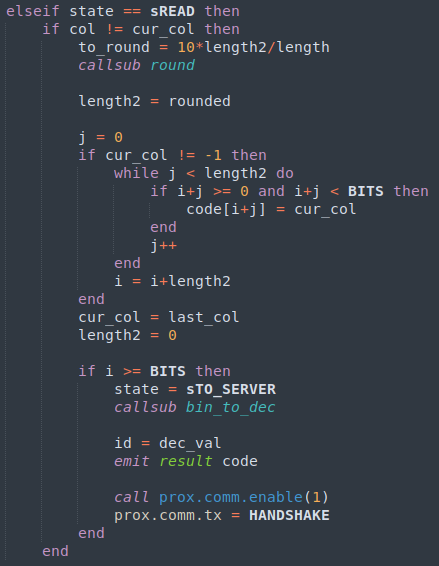
\includegraphics[width=0.7\linewidth]{code/client_barcode_reading}
  \caption{Lecture du code-barres (Aseba)}
  \label{fig:client_barcode_reading}
\end{figure}

\subsection{Communication}
\label{sec:communication}
Cette brève section à pour but d'expliquer les bases du protocole de communication. Pour une meilleur compréhension, veuillez vous référer à l'annexe \ref{app:protocol}.

L'environnement Aseba permet de transmettre des valeurs de 10 bits d'un robot à l'autre via les capteurs de proximité, c'est à dire un nombre entre 0 et 1023 inclus.
Nous avons décidé d'utiliser 4 bits pour définir la commande et les 6 autres pour les données associées.

Prenons l'exemple de la commande "send id", envoyée par le client pour transmettre son identifiant au serveur. L'id de la commande est $2_d$ ou $0010_b$\footnote{$x_d$ est la représentation décimale et $x_b$ la représentation binaire}.

Pour former le message complet, il faut décaler ce nombre de 6 bits vers la gauche pour laisser la place aux 6 bits de données. En Aseba, comme dans de nombreux langages, l'opérateur de décalage binaire est \texttt{<<} suivi du nombre de bits à décaler.

Ainsi,
\[ 2_d = 0010_b \]
\[ 2_d << 6 = 0010_b << 6 = 00\ 1000\ 0000_b = 128_d \]

On y ajoute l'identifiant du robot convertit en décimal. Cet identifiant étant encodé sur 6 bits, il est limité à une valeur inférieure ou égale à 63. Prenons l'id $43_d$ ($10\ 1011_b$), on a donc:

\[\begin{array}[t]{r}
   00\ 1000\ 0000 \\
+\ 00\ 0010\ 1011 \\ \hline
   00\ 1010\ 1011
\end{array}
\]

Le client $43_d$ voulant communiquer son identifiant au serveur enverra donc le message $00\ 1010\ 1011$.

Pour décoder un message reçu, le processus est très simple. Continuons avec notre exemple mais du point de vue du serveur.

Pour extraire la commande, il suffit de redécaler le message vers la droite de 6 bits. Ainsi,
\[\begin{array}[t]{r}
   00\ 1010\ 1011\ (>> 0)\\
    0\ 0101\ 0101\ (>> 1)\\
       0010\ 1010\ (>> 2)\\
        001\ 0101\ (>> 3)\\
         00\ 1010\ (>> 4)\\
          0\ 0101\ (>> 5)\\
             0010\ (>> 6)
\end{array}
\]

on retrouve bien $0010_b = 2_d$, la commande "send id".

Pour isoler les données, on peut utiliser ce qui s'appelle un masque avec l'opération "et" binaire. L'opérateur \binampersand (ou "et" binaire) applique la table de vérité suivante sur chaque les bits de deux nombres deux à deux.

\begin{center}
  \begin{tabular}{|c|c||c|}
    \hline
    $A$ & $B$ & $A \binampersand B$ \\
    \hline
    $0$ & $0$ & $0$ \\
    \hline
    $0$ & $1$ & $0$ \\
    \hline
    $1$ & $0$ & $0$ \\
    \hline
    $1$ & $1$ & $1$ \\
    \hline
  \end{tabular}
\end{center}

Pour conserver les 6 bits les moins significatifs (càd à droite), il faut faire $message\ \binampersand\ 11\ 1111_b$, dans notre cas, \[
\begin{array}[t]{r}
               00\ 1010\ 1011 \\
\binampersand\ 00\ 0011\ 1111 \\ \hline
               00\ 0010\ 1011
\end{array}
\]

On obtient ainsi $10\ 1011_b = 43_d$, l'identifiant du client.

\pagebreak

\section{Côté serveur}
Le programme côté serveur est séparé en 2 parties qui sont respectivement séparées en 2 et 4 états.
\subsection{Communication}
La section communication est séparée en 2 états. Le premier consiste uniquement à attendre de recevoir un handshake (cf. annexe \ref{app:communication}) et de passer à l'état suivant qui lui s'occupe de toute la partie échange d'informations.\\
Les échanges sont gérés par cette section du programme:

\begin{figure}[h]
	\centering
	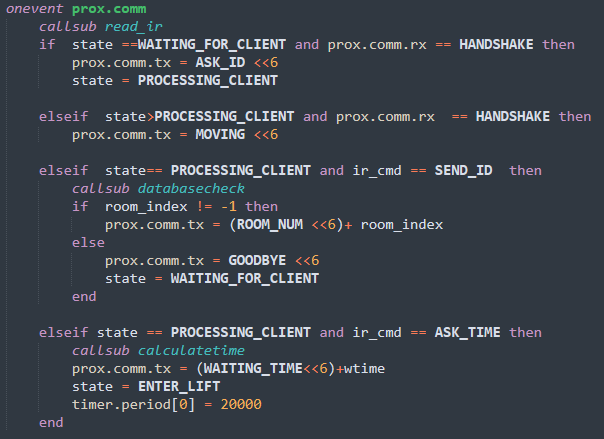
\includegraphics[scale=0.5]{code/server_decodage}
	\caption{Partie communication}
	\label{fig:decodage}
\end{figure}

On peut voir qu'il y a un appel à la sous-routine nommée \texttt{databasecheck}. Cette sous-routine s'occupe de tout ce qui concerne la database, qui est une liste avec 16 éléments représentant les 16 chambres. Si la valeur est de -1 la chambre est libre et si la chambre est occupé, le numéro du client remplace le -1.
La numérotation des chambres choisie est celle-ci:
\begin{center}
	\begin{tabular}{|c|c|c|c|}
		\hline
		12&13  &14  &15  \\
		\hline
		8&9  &10  &11  \\
		\hline
		4&5  &6  &7  \\
		\hline
		0&1  &2  &3  \\
		\hline
	\end{tabular}
\end{center}
Nous avons opté pour cette numérotation car elle nous permet de facilement récupérer les coordonées de la chambres comme ceci:
\begin{figure}[h]
	\centering
	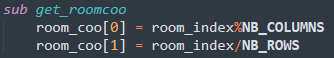
\includegraphics{code/server_roomcoo}
	\caption{Coordonées de la chambre}
	\label{fig:roomcoo}
\end{figure}

Voici un schéma de la fonction \texttt{databasecheck}:

\begin{figure}[h]
	\centering
	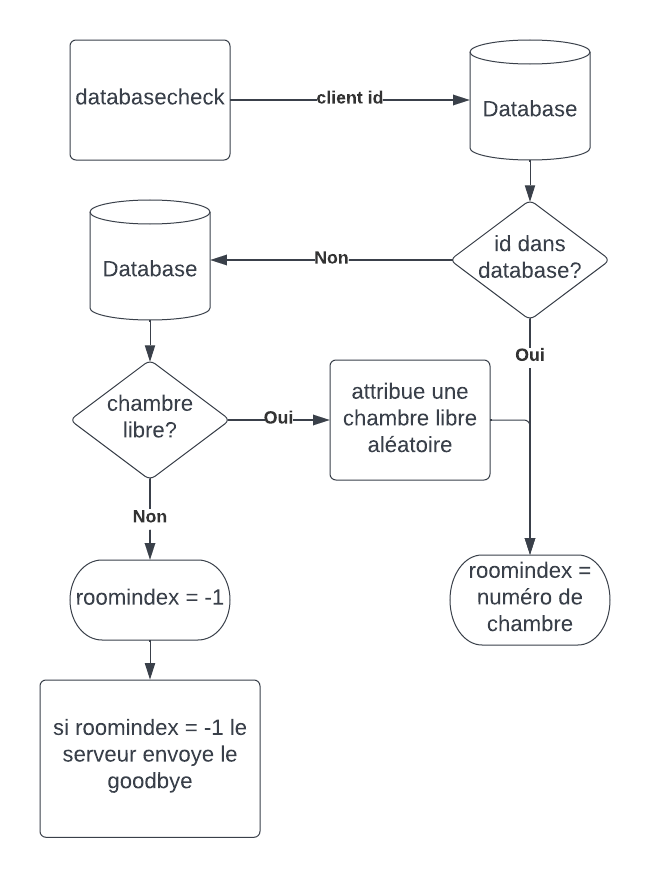
\includegraphics[scale=0.25]{code/server_databasecheck}
	\caption{Schéma de la sous-routine \texttt{databasecheck}}
	\label{fig:schéma database}
\end{figure}

Le code en aseba de cette fonction est disponible dans l'annexe \ref{app:databasecheck}.

Une fois la communication terminée le serveur laisse 20 secondes au client pour entrer dans l'ascenseur, après quoi la fonction \texttt{start\_moving} est appelée.

Cette fonction est utilisée pour initialiser les différentes valeurs (\texttt{htime}, \texttt{vtime}, \texttt{hor}, \texttt{ver}, \texttt{direction}). L'ascenseur commence par aller à l'horizontale puis à la verticale et pour le retour, le mouvement est inversé. Nous avons dû utiliser le temps moyen par étage/colonne car en aseba les nombres sont des entiers signés sur 16 bits (valeur maximum de 32767) et que les \texttt{timers} sont en millisecondes celà nous laisse un timer maximum de 32 secondes or, nous dépassons ce temps.

Voici la fonction en question avec une fonction similaire pour le retour:

\begin{figure}[h]
	\centering
	%pour aligner
	\raisebox{-0.5\height}{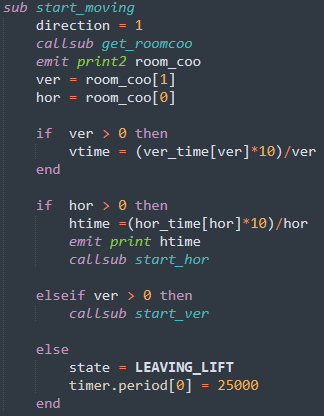
\includegraphics[scale=0.7]{code/server_startmoving}}
	\raisebox{-0.5\height}{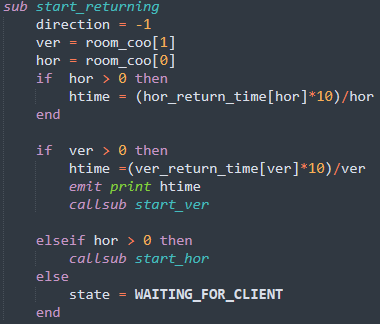
\includegraphics[scale=0.7]{code/server_startreturning}}
	\caption{Fonction \texttt{start\_moving} et \texttt{start\_returning}}
	\label{fig:startmoving}
\end{figure}

Les temps verticaux et horizontaux d'aller et de retour ont été calculés grâce au programme de calibration (\texttt{calibration.aesl})

Les fonctions \texttt{start\_ver} et \texttt{start\_hor} servent uniquement à démarrer les moteurs et lancer les \texttt{timers}. La variable direction sert à changer entre l'aller (= 1) et le retour (= -1).

Voici ce que celà donne en aseba:

\begin{figure}[H]
	\centering
	%pour aligner
	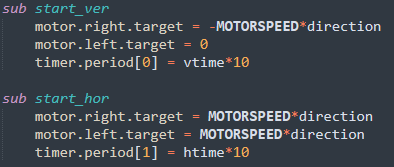
\includegraphics{code/server_direction_moving}
	\caption{Fonction \texttt{start\_ver} et \texttt{start\_hor}}
	\label{fig:startdirection}
\end{figure}

Ensuite tout le reste du déplacement se déroule dans les \texttt{timers}. Le \texttt{timer0} sert au mouvement vertical et le \texttt{timer1} l'horizontal. Le \texttt{timer0} s'occupe aussi de tous les autres moments d'attente (entrée et sortie de l'ascenseur).

À la fin de l'aller l'ascenseur laisse 25 secondes au client pour sortir avant de repartir. Une fois l'ascenseur retourné au point de départ le serveur est prêt à recevoir un nouveau client.

Lorsque le serveur est occupé à déplacer l'ascenseur et qu'un nouveau client arrive, il lui envoie un message pour lui dire d'attendre.
